\documentclass[journal,twoside,web]{ieeecolor}
\usepackage{generic}
\usepackage{cite}
\usepackage{amsmath,amssymb,amsfonts}
\usepackage{algorithmic}
\usepackage{graphicx}
\usepackage{algorithm,algorithmic}
\usepackage{hyperref}
\hypersetup{hidelinks=true}
\usepackage{textcomp}
\usepackage[utf8]{inputenc} % Kodowanie UTF-8
\usepackage[T1]{fontenc}    % Poprawne kodowanie fontów
\usepackage{polski}         % Wsparcie dla języka polskiego
\usepackage[polish]{babel}  % Polskie reguły typograficzne
\usepackage{float}
\usepackage{setspace}


% Zmiana etykiety Fig. na Rysunek
\addto\captionspolish{\renewcommand{\figurename}{Rysunek}}

\def\BibTeX{{\rm B\kern-.05em{\sc i\kern-.025em b}\kern-.08em
    T\kern-.1667em\lower.7ex\hbox{E}\kern-.125emX}}
\markboth{\hskip25pc IEEE TRANSACTIONS AND JOURNALS TEMPLATE}
{Author \MakeLowercase{\textit{et al.}}: Title}

\begin{document}
\title{Regulatory niecałkowitego rzędu w manipulatorach}

\author{}

\maketitle
\onehalfspacing

\section{Streszczenie}
W artykule przedstawiono zastosowanie rachunku różniczkowego niecałkowitego rzędu w projektowaniu układów sterowania manipulatorami o sześciu stopniach swobody. Omówiono teoretyczne podstawy tego podejścia oraz narzędzia wykorzystywane do modelowania i symulacji, takie jak MATLAB, Simulink, Simscape, FOMCON, Robotics Toolbox i ROS2. Szczególną uwagę poświęcono regulatorowi niecałkowitego rzędu. Wyniki badań wskazują na potencjał rachunku niecałkowitego rzędu w zaawansowanych zastosowaniach robotycznych.

\section{Wstęp}
\label{sec:introduction}
\IEEEPARstart{R}{achunek} niecałkowitego rzędu, rozwijany na przestrzeni ostatnich dekad, zyskuje na znaczeniu w obszarze inżynierii sterowania. Dzięki swojej elastyczności i możliwości modelowania systemów z pamięcią, stanowi doskonałe narzędzie do opisu i projektowania układów o złożonej dynamice. W porównaniu z klasycznym rachunkiem różniczkowym, oferuje on możliwość dostosowania charakterystyki dynamicznej układów poprzez precyzyjną manipulację rzędami pochodnych i całek, co otwiera nowe kierunki w optymalizacji i analizie systemów sterowania. Podstawy rachunku i jego zastosowania w elektrotechnice, automatyce i teorii sterowania są szeroko opisane, przez specjalistów w dziedzinie \cite{Fractional, Selected, Pawlusz, Popolizio}.  

Praktyczne zastosowania układów niecałkowitego rzędu obejmują szeroki wachlarz dziedzin, takich jak sterowanie procesami przemysłowymi, modelowanie dynamiczne w biologii czy inżynieria mechaniczna \cite{Kumar, plant, falling, power}. W kontekście układów sterowania, rozwiązania te pozwalają na zwiększenie dokładności regulacji, redukcję przeregulowań i poprawę tłumienia zakłóceń.

Celem niniejszego artykułu jest analiza zastosowania rachunku niecałkowitego rzędu w projektowaniu układów sterowania manipulatora o sześciu stopniach swobody. W pracy przedstawiono metody oraz narzędzia użyte w procesie modelowania i symulacji. Szczególny nacisk położono na wykorzystanie oprogramowania MATLAB i Simulink, które umożliwiły przeprowadzenie symulacji oraz obliczeń numerycznych.

Biblioteka Simscape, będąca częścią środowiska Simulink, zapewniła możliwość szybkiego i efektywnego tworzenia modeli elektrycznych, mechanicznych oraz mechatronicznych systemów wielodziedzinowych. Do modelowania i analizy układów niecałkowitego rzędu wykorzystano bibliotekę FOMCON, która oferuje zaawansowane narzędzia do projektowania i symulacji takich systemów.

W kontekście robotyki zastosowano Robotics Toolbox, który umożliwił przeprowadzanie operacji na modelach manipulatora, w tym analizę kinematyki i dynamiki. Dodatkowo, wykorzystano system ROS2 (Robot Operating System 2), który pozwala na modułowe projektowanie i prototypowanie systemów robotycznych. Komunikację na odległość z systemem ROS2 zrealizowano za pomocą Hamachi, zapewniającego bezpieczne połączenie przez VPN.

Integracja symulacji z ROS2 została osiągnięta dzięki ROS Toolbox, który umożliwił przesyłanie danych między Simulinkiem a ROS2, a także stworzenie zdalnej wizualizacji ruchu manipulatora. Przedstawione narzędzia i metody stanowią kompleksowe podejście do projektowania i analizy zaawansowanych układów sterowania manipulatorów, podkreślając zalety wykorzystania rachunku niecałkowitego rzędu. 
\section{Metody}
\subsection{Matlab i Simulink}
MATLAB to zaawansowane środowisko obliczeniowe, które umożliwia przeprowadzanie analiz numerycznych, przetwarzanie danych, modelowanie matematyczne oraz wizualizację wyników. Jego wszechstronność i szeroka gama funkcji sprawiają, że jest wykorzystywany w wielu dziedzinach, takich jak inżynieria, nauki ścisłe czy finanse. MATLAB wspiera użytkownika poprzez gotowe biblioteki i narzędzia, które upraszczają implementację zaawansowanych algorytmów i umożliwiają szybkie prototypowanie rozwiązań. \href{https://www.mathworks.com/help/matlab/}{\cite{matlab}}

Simulink to rozszerzenie MATLAB-a dedykowane modelowaniu, symulacji i analizie systemów dynamicznych. Dzięki graficznemu interfejsowi użytkownika umożliwia intuicyjne tworzenie modeli za pomocą bloków reprezentujących elementy systemu, co znacząco przyspiesza proces projektowania. Simulink jest szczególnie ceniony w automatyce, robotyce oraz przemyśle motoryzacyjnym, gdzie znajduje zastosowanie w projektowaniu i testowaniu systemów sterowania, przetwarzaniu sygnałów czy analizie systemów mechatronicznych. \href{https://www.mathworks.com/help/simulink/}{\cite{simulink}}

\subsection{FOPID}
Regulator FOPID (ang. Fractional-Order Proportional-Integral-Derivative) jest rozszerzeniem klasycznego regulatora PID, który wykorzystuje pojęcia rachunku różniczkowego i całkowego niecałkowitego rzędu. W przeciwieństwie do standardowego PID, gdzie działania różniczkowania i całkowania są określone jako operatory pierwszego i zerowego rzędu, w FOPID ich rzędy są dowolnymi liczbami rzeczywistymi, oznaczonymi jako $\lambda$ (rząd całkowania) oraz $\mu$ (rząd różniczkowania) \eqref{eq:FOPID}.
\begin{equation}
	G(s) = K_{p} + \frac{K_{i}}{s^{\lambda}} + K_{d}s^{\mu}
	\label{eq:FOPID}
\end{equation} 
Przedstawiane badania wykorzystują bibliotekę FOMCON, opisaną w sekcji E. 
\subsection{Robotics Toolbox}
Robotics Toolbox to biblioteka dostępna dla MATLAB-a, zaprojektowana z myślą o analizie, symulacji i projektowaniu systemów robotycznych. Narzędzie to dostarcza zestawu funkcji i obiektów wspomagających modelowanie manipulatorów, pojazdów mobilnych oraz systemów autonomicznych, umożliwiając kompleksowe badania nad różnymi aspektami robotyki. Główne funkcjonalności Robotics Toolbox obejmują:

\begin{itemize}
	\item modelowanie manipulatorów – definiowanie struktur kinematycznych i dynamicznych przy użyciu reprezentacji Denavita-Hartenberga (DH) lub standardu URDF,
	\item kinematykę – analiza kinematyki prostej i odwrotnej manipulatorów,
	\item planowanie trajektorii – generowanie trajektorii ruchu manipulatorów i pojazdów mobilnych w przestrzeni operacyjnej,
	\item symulację i wizualizację – możliwość symulowania ruchu robotów oraz wizualizacji 3D,
	\item analizę dynamiki – symulacja sił i momentów działających w systemach robotycznych.
\end{itemize}
Robotics Toolbox wspiera badania nad algorytmami sterowania, umożliwia testowanie nowych metod planowania ruchu oraz integrację z innymi narzędziami, takimi jak Simulink czy ROS. Dzięki swoim wszechstronnym możliwościom, jest szczególnie ceniony w projektach badawczo-rozwojowych i edukacji z zakresu automatyki i robotyki. \href{https://www.mathworks.com/help/robotics/}{\cite{Robotics Toolbox}}
\subsection{Simscape}
Simscape to narzędzie rozszerzające możliwości MATLAB-a i Simulinka, które umożliwia modelowanie, symulację oraz analizę systemów fizycznych w sposób intuicyjny, za pomocą komponentów graficznych. Jest szczególnie przydatne w dziedzinach, gdzie systemy mają złożoną strukturę wielodomenową, łączącą elementy mechaniczne, elektryczne, hydrauliczne czy termiczne \href{https://www.mathworks.com/help/robotics/}{\cite{Simscape}}. Główne cechy Simscape:
\begin{itemize}
	\item modelowanie wielodomenowe – możliwość integracji elementów z różnych dziedzin fizyki w jednym środowisku symulacyjnym,
	\item komponenty gotowe do użycia – bogata biblioteka bloków reprezentujących elementy, takie jak rezystory, silniki, zawory czy tłoki,
	\item podejście opierające się na fizyce – modele bazują na rzeczywistych równaniach opisujących zjawiska fizyczne, co ułatwia dokładne odwzorowanie systemów,
	\item symulacja dynamiczna – możliwość analizowania zachowań systemów w czasie, z uwzględnieniem nieliniowości i sprzężeń między domenami.
\end{itemize}
\subsection{FOMCON}
FOMCON jest biblioteką Matlaba i Simulinka, która wprowadza do środowisk możliwość dodania numerycznej implementacji układów regulacji bazujących na funkcjach niecałkowitego rzędu. Biblioteka bazuje na definicji dyskretnej Grünwald'a–Letnikov'a \eqref{eq:GL}.

\begin{equation}
	\Delta ^{\alpha}x_{k} = \sum_{j=0}^{k}(-1)^{j}\left( 
	\begin{matrix}
		\alpha \\
		j
	\end{matrix}\right) x_{k-j}
	\label{eq:GL}
\end{equation}

Do odtwarzania wyników ciągu dyskretnego - w bibliotece - wykorzystywana jest aproksymacja Oustaloupa, która jest budowana na podstawie transmitancji operatorowej rachunku, w zdefiniowanym zakresie częstotliwości i ograniczeniu pamięci próbek \textit{N} \eqref{eq:Oustaloup}.
\begin{equation}
	s^{\alpha} = G_{\omega} \prod_{k=-N}^{N}\frac{s + \omega_{k}'}{s + \omega_{k}}
	\label{eq:Oustaloup}
\end{equation}
Szczegóły transformacji i aproksymacji są dokładniej opisane przez autorów biblioteki \cite{FOMCON,FOMCONdoc}. Gotowy blok regulatora; Fig \ref{fig:fopid}; niecałkowitego rzędu może zostać wstawiony bezpośrednio do wcześniej przygotowanych modeli.

\begin{figure}[H]
	\centering
	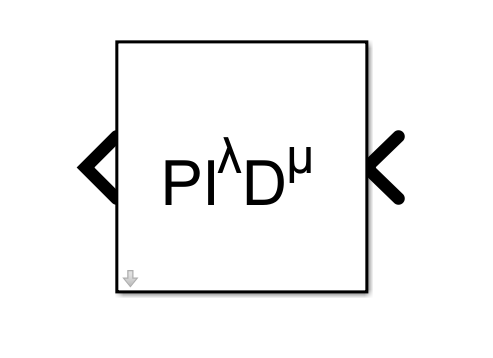
\includegraphics[width=0.7\linewidth]{../figs/FOPID}
	\caption{Blok regulatora FOPID}
	\label{fig:fopid}
\end{figure}

Wewnątrz bloku można określić parametry tj.:

\begin{itemize}
	\item wzmocnienie proporcjonalne $K_{p}$,
	\item wzmocnienie całkowania $K_{i}$,
	\item rząd całkowania $\lambda$,
	\item wzmocnienie różniczkowania $K_{d}$,
	\item rząd różniczkowania $\mu$,
	\item zakres częstotliwości aproksymacji,
	\item rząd aproksymacji. 
\end{itemize}
\subsection{ROS2}
Robot Operating System 2 (ROS2) to otwarte środowisko programistyczne zaprojektowane do tworzenia aplikacji dla systemów robotycznych. Stanowi rozwinięcie pierwotnej wersji ROS, wprowadzając znaczące ulepszenia w zakresie wydajności, skalowalności oraz bezpieczeństwa. ROS2 umożliwia projektowanie systemów modularnych, które mogą działać na wielu platformach, takich jak Linux, Windows czy macOS, a także na urządzeniach wbudowanych. Dzięki wsparciu dla komunikacji typu publish-subscribe, ROS2 pozwala na efektywną wymianę danych pomiędzy komponentami systemu robotycznego \href{https://docs.ros.org/en/foxy/index.html}{\cite{ROS2}}. 

Wizualizacja manipulatora została stworzona w aplikacji RVIZ systemu ROS2. 
\subsection{Hamachi}

Hamachi to narzędzie do tworzenia wirtualnych sieci prywatnych (VPN), które umożliwia bezpieczne połączenie komputerów przez internet, tak jakby znajdowały się one w tej samej lokalnej sieci. Jest to rozwiązanie typu peer-to-peer, często używane do zdalnej gry, pracy zespołowej i w sytuacjach, gdy tradycyjne rozwiązania VPN są zbyt skomplikowane lub kosztowne. Połączenia w Hamachi są szyfrowane, co zapewnia bezpieczeństwo przesyłanych danych. Umożliwia to dostęp do zasobów w sieci lokalnej, nawet jeśli komputery znajdują się w różnych miejscach na świecie. Hamachi działa bez potrzeby ręcznej konfiguracji routerów, co upraszcza połączenie w środowiskach, w których nie ma pełnej kontroli nad ustawieniami sieciowymi. Może być używane do współpracy na plikach i aplikacjach działających w sieci lokalnej, a także do dostępu do urządzeń, takich jak drukarki czy kamery sieciowe. Umożliwia także zdalny dostęp do zasobów firmowych lub domowych. Hamachi działa na systemach Windows, macOS i Linux, a jego wersja podstawowa jest bezpłatna, z ograniczeniem liczby użytkowników w wirtualnej sieci. Dla większej liczby połączeń dostępna jest wersja płatna. W artykule sieć VPN została wykorzystana do przesyłania pozycji stawów i wizualizacji procesu, symulacji manipulatora w RVIZ dostępnym wraz z systemem ROS2. W systemie opartym na Linux, tj. Ubuntu Desktop Hamachi nie posiada GUI. Żeby zaimplementować interfejs graficzny należy pobrać Haguichi (GUI Hamachi w Ubuntu) \href{https://haguichi.net/download/}{\cite{Haguichi}}.
Proces instalacji dla systemu Ubuntu, Linux Mint i innych systemów pochodnych:

\begin{footnotesize}
\begin{verbatim}
	sudo add-apt-repository -y ppa:ztefn/haguichi-stable
	sudo apt update
	sudo apt install -y haguichi
\end{verbatim}
\end{footnotesize}
\subsection{ROS Toolbox}

ROS Toolbox \href{https://www.mathworks.com/help/ros/}{\cite{ROS Toolbox}} to narzędzie dostępne w MATLAB, które umożliwia integrację z systemami opartymi na Robot Operating System (ROS) oraz ROS 2. Ułatwia projektowanie, symulację i analizę algorytmów dla systemów robotycznych, a także pozwala na komunikację z rzeczywistymi robotami. Toolbox oferuje funkcje takie jak wysyłanie i odbieranie wiadomości ROS, subskrypcję tematów, wywoływanie usług i akcji, a także generowanie niestandardowych typów wiadomości. Umożliwia również symulację i wizualizację za pomocą narzędzi takich jak Gazebo czy Rviz oraz integrację z Simulink. Blok Publishera umożliwia wysyłanie danych środowiska Simulink; w tym wypadku przez VPN; do systemu ROS2; Rysunek \ref{fig:pub}.
\begin{figure}[H]
	\centering
	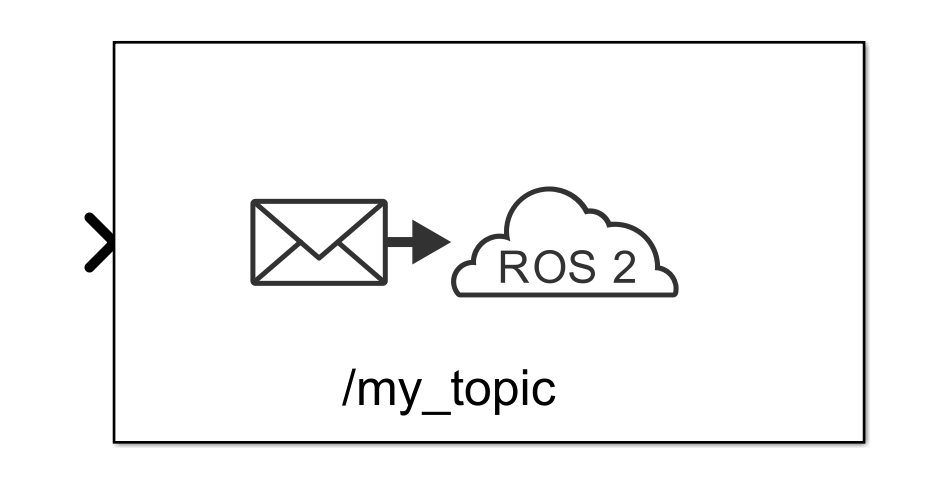
\includegraphics[width=0.7\linewidth]{../figs/pub}
	\caption{Blok publikujący na temacie}
	\label{fig:pub}
\end{figure}
Blok odbierający dane z tematu; Rysunek \ref{fig:sub}; odbiera dane, które zwraca system ROS2 (nasłuchuje danych na określonym temacie).
\begin{figure}[H]
	\centering
	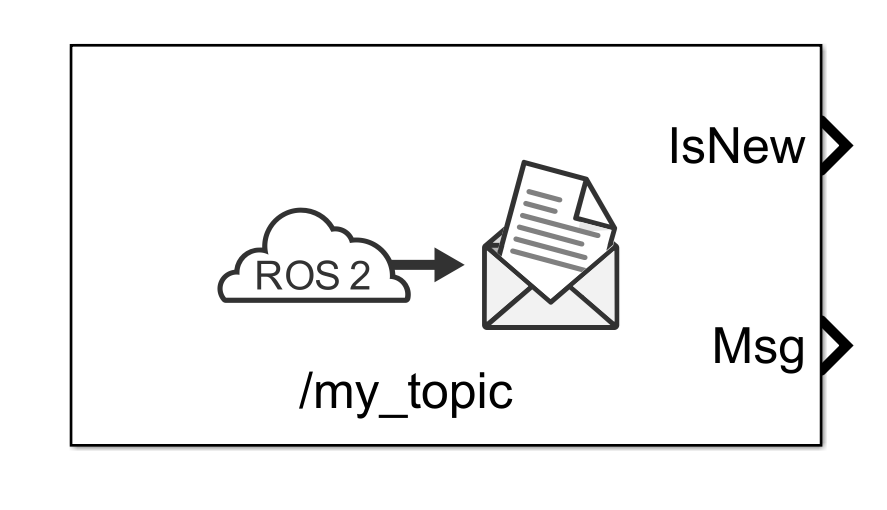
\includegraphics[width=1\linewidth]{../figs/sub}
	\caption{Subskrybent w Simulinku}
	\label{fig:sub}
\end{figure}

\subsection{Model Manipulatora}
Modele 3D elementów manipulatora zostały opracowane w programie Fusion 360. Następnie zostały zaimportowane do środowiska Simulink, gdzie przeprowadzono ich odpowiednie rozmieszczenie, uwzględniając także właściwości inercyjne oraz parametry materiałowe poszczególnych elementów robota. W rezultacie tych działań uzyskano implementację modelu matematycznego manipulatora, gotowego do dalszej analizy i symulacji. 
\begin{figure}[H]
	\centering
	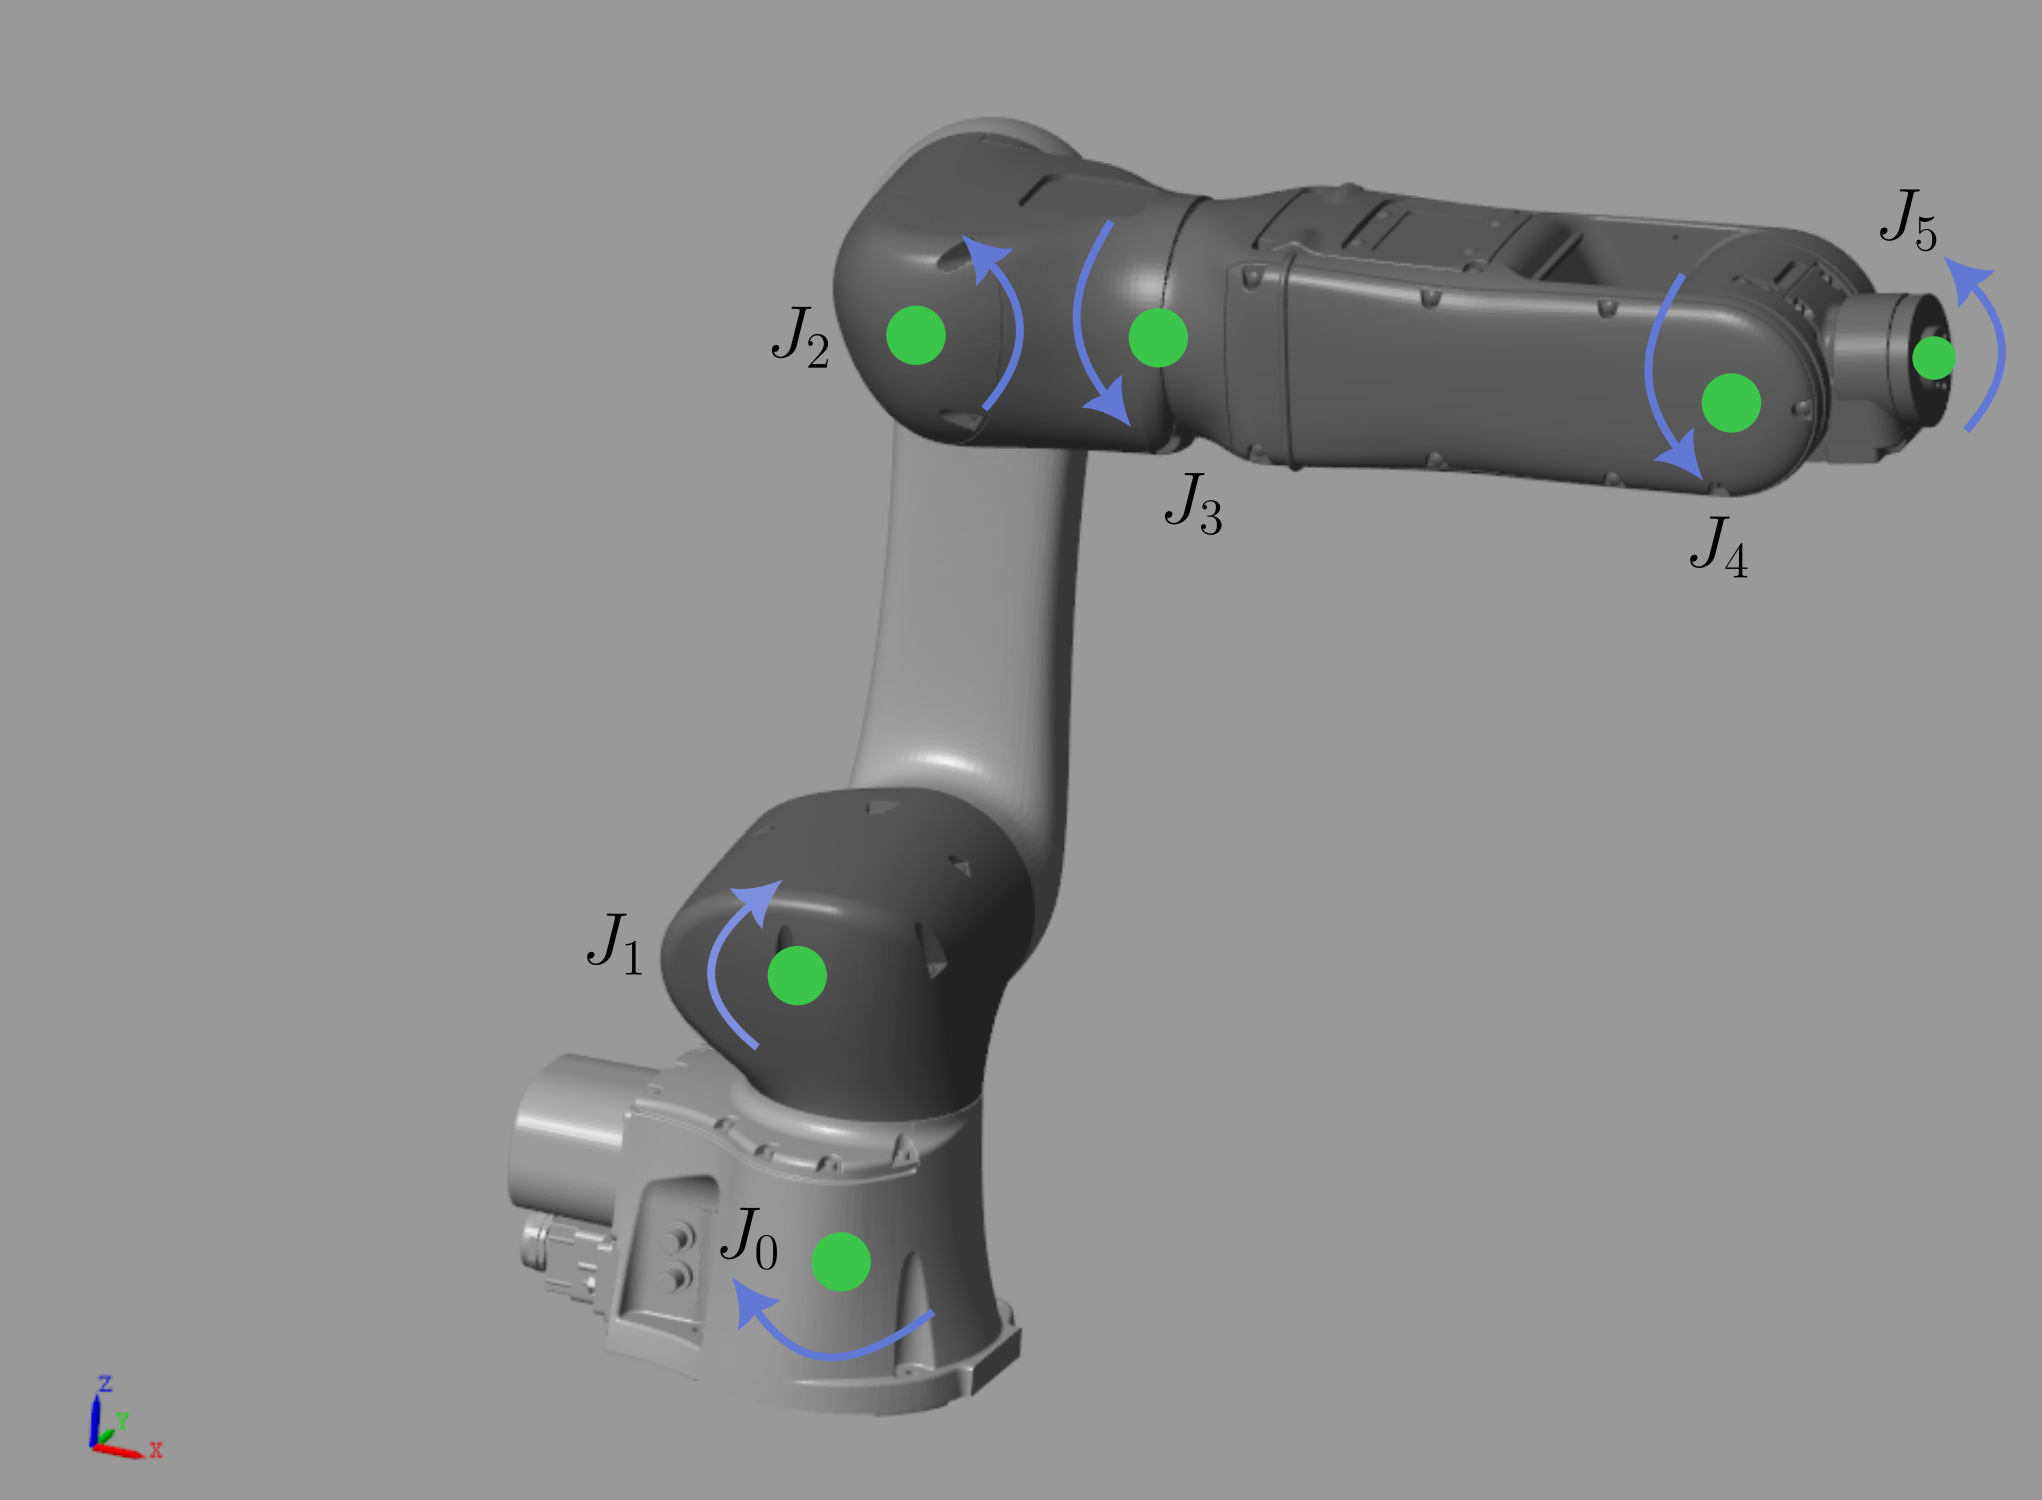
\includegraphics[width=1\linewidth]{../figs/joints}
	\caption{Model 3D manipulatora}
	\label{fig:joints}
\end{figure}
Robot posiada 6 stawów typu revolute, co implikuje ruch o sześciu stopniach swobody. Układ sterowania; Fig \ref{fig:ster} został zbudowany w oparciu o technikę kaskadowych układów regulacji. Nadrzędną pętlę stanowi układ regulacji położenia kątowego. Wyjściem regulatora położenia jest zadana prędkość kątowa, która reaguje w pętli podrzędnej z regulatorem prędkości kątowej. Dla każdego stawu układ regulacji został skopiowany sześciokrotnie. Podczas tworzenia modelu nie zostały uwzględnione modele układów napędowych, ponieważ wtedy poziom skomplikowania i czas budowy modelu zdecydowanie by się wydłużył. Dynamika samych napędów nie ma wpływu na przeprowadzane badanie.
\begin{figure*}[hbt!]
	\centering
	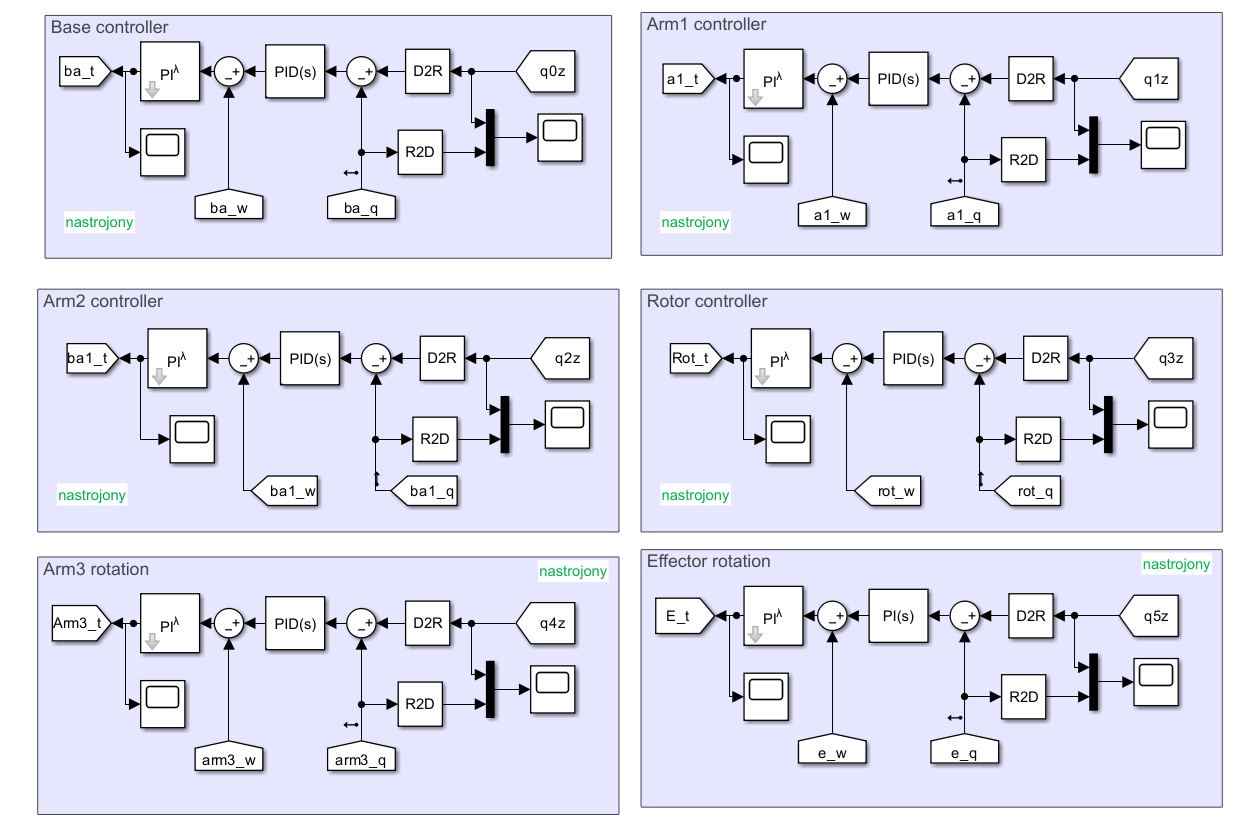
\includegraphics[width=1\linewidth]{../figs/ster}
	\caption{Układ sterowania położeniem kątowym stawów manipulatora}
	\label{fig:ster}
\end{figure*}
 
\subsection{Proces strojenia regulatorów}

Ręczne strojenie większego, nieliniowego modelu z początku może wydawać się skomplikowane jednak w tym rozdziale zostaną zestawione; empiryczne spostrzeżenia związane z całym procesem. Na początku trzeba ustawić wartości wzmocnień tak, aby regulatory utrzymywały się samoistnie w początkowym położeniu równowagi lub mechanicznie zablokować położenie wszystkich stawów. Strojenie rozpoczyna się od stawu końcowego, ponieważ układ regulacji położenia efektora jest najmniej zależny od dynamiki pozostałych członów robota. Proces ręcznego doboru nastaw powinien się rozpocząć od pętli wewnętrznych (prędkości kątowych). Na wyjściu układ zapewnia moment, który powinien przezwyciężyć opory ruchu i aperiodycznie doprowadzić do osiągnięcia zadanego położenia. Nadrzędne układy regulacji muszą zawierać regulatory PID, ponieważ z tego co zostało zauważone podczas strojenia, jeśli dynamika członu zależy również od innego, niezależnego członu, żeby przeciwdziałać szybkim zmianom i ewentualnym drganiom robota, potrzebny jest człon różniczkujący, który zapewni dużą reakcję na szybkie zmiany położenia układu. Po procesie strojenia można przejść do wykonania właściwych badań. Nastrojone układy regulacji całkowitego rzędu stanowią część porównawczą badań. 
\section{Wyniki}
W bieżącym rozdziale szczegółowo omówiono wyniki badań dotyczących wpływu zastosowania regulatorów niecałkowitego rzędu w podrzędnej pętli regulacji prędkości kątowej stawów. Celem tych badań było porównanie efektywności regulatorów niecałkowitego rzędu z klasycznymi regulatorami całkowitego rzędu. W trakcie eksperymentów, podczas modulacji rzędu regulatorów, nie zmieniano nastaw samych regulatorów, co pozwoliło na zachowanie spójności parametrów i umożliwiło bezpośrednie porównanie charakterystyk dynamicznych całego układu. W ten sposób badano, jak zmiana rzędu regulatorów wpływa na stabilność i dokładność śledzenia zadanej nieliniowej trajektorii w układzie regulacji. 

\subsection{Charakterystyki częstotliwościowe regulatorów}

Zadanie sinusoidalnie zmieniającego się położenia kątowego, dla każdego ze stawów prowadzi do realizacji nieliniowej trajektorii. Amplituda sinusoidy wynosząca 10 stopni rozszerza zakres badanych częstotliwości, umożliwiając analizę systemu w szerszym zakresie dynamiki. Stosunek otrzymanej do zadanej amplitudy zmiany położenia kątowego dla pięciu znaczących ramion i różnych rzędów całkowania w stanie ustalonym, pod względem częstotliwości zestawiają Tabele \ref{tab:lam1}.
W miejscach, gdzie zamiast wyników pojawiają się myślniki, oznacza to, że dany człon układu nie był stabilny, nie osiągał wymaganej wartości zadanej lub z powodu specyfiki jego działania występowała składowa zerowa. Ta składowa uniemożliwiała poprawne odwzorowanie sygnału zadanego, co mogło prowadzić do braku pełnej realizacji oczekiwanego przebiegu. W Tabeli \ref{tab:lam1}, przy częstotliwości 4 Hz, odczytanie wartości amplitudy nie jest możliwe ze względu na występowanie znaczącej składowej zerowej, która uniemożliwia odtworzenie wartości zadanej. 
\begin{table}[h]
	\centering
	\caption{Charakterystyka częstotliwościowa dla $\lambda$ = 1}
	\label{tab:lam1} % Dodanie etykiety
	\begin{tabular}{|c|c|c|c|c|c|}
		\hline
		$f_z$ & $\frac{I_{0}}{I_z}$ & $\frac{I_{1}}{I_z}$ & $\frac{I_{2}}{I_z}$ & $\frac{I_{3}}{I_z}$ & $\frac{I_{4}}{I_z}$ \\
		\hline
		Hz & - & - & - & - & - \\
		\hline
		$\frac{1}{50}$ & 1 & 0.96 & 1 & 1 & 1 \\
		\hline
		$\frac{1}{40}$ & 1 & 0.96 & 1 & 1 & 1 \\
		\hline
		$\frac{1}{30}$ & 1 & 0.96 & 0.95 & 1 & 0.95 \\
		\hline
		$\frac{1}{20}$ & 1 & 0.96 & 0.92 & 1 & 0.94 \\
		\hline
		$\frac{1}{10}$ & 1 & 0.96 & 0.92 & 1 & 0.94 \\
		\hline
		$\frac{1}{5}$ & 1 & 0.97 & 0.92 & 0.96 & 0.96 \\
		\hline
		$\frac{1}{4}$ & 0.98 & 0.97 & 0.94 & 0.94 & 0.97 \\
		\hline
		$\frac{1}{3}$ & 0.95 & 0.97 & 0.95 & 0.94 & 0.98 \\
		\hline
		$\frac{1}{2}$ & 0.86 & 0.97 & 0.96 & 0.91 & 1.02 \\
		\hline
		1 & 0.76 & 0.97 & 0.90 & 0.87 & 0.92 \\
		\hline
		2 & 0.76 & 0.97 & 0.74 & 0.78 & 0.60 \\
		\hline
		3 & 0.72 & 0.94 & 0.67 & - & 0.40 \\
		\hline
		4 & - & - & - & - & - \\
		\hline
	\end{tabular}
\end{table}
Badanie dla $\lambda$ = 0.5 ogranicza się do jeszcze mniejszych częstotliwości sygnałów zadanych; Tabela \ref{tab:lam05}. Zmniejszenie rzędu całkowania dodatkowo ogranicza możliwości odtworzenia sygnału zadanego przez układ. Ograniczenie rzędu całkowania w pętli regulacji prędkości kątowej zmniejsza możliwość do odtworzenia momentu zadanego na wyjściu regulatora, w wyniku czego zwiększa się błąd składowej stałej i zmniejsza stabilność układu dla większych częstotliwości.  
\begin{table}[h]
	\centering
	\caption{Charakterystyka częstotliwościowa dla $\lambda$ = 0.5}
	\label{tab:lam05} % Dodanie etykiety
	\begin{tabular}{|c|c|c|c|c|c|}
		\hline
		$f_z$ & $\frac{I_{0}}{I_z}$ & $\frac{I_{1}}{I_z}$ & $\frac{I_{2}}{I_z}$ & $\frac{I_{3}}{I_z}$ & $\frac{I_{4}}{I_z}$ \\
		\hline
		Hz & - & - & - & - & - \\
		\hline
		$\frac{1}{50}$ & 1 & 0.96 & 0.95 & 1 & 1 \\
		\hline
		$\frac{1}{40}$ & 1 & 0.96 & 0.97 & 1 & 0.95 \\
		\hline
		$\frac{1}{30}$ & 1 & 0.96 & 0.97 & 1 & 0.95 \\
		\hline
		$\frac{1}{20}$ & 1 & 0.96 & 0.97 & 1 & 0.94 \\
		\hline
		$\frac{1}{10}$ & 1.1 & 0.96 & 0.97 & 1 & 0.94 \\
		\hline
		$\frac{1}{5}$ & 1 & 0.97 & 0.93 & 0.96 & 0.96 \\
		\hline
		$\frac{1}{4}$ & 0.98 & 0.97 & 0.94 & 0.95 & 0.98 \\
		\hline
		$\frac{1}{3}$ & 0.95 & 0.98 & 0.95 & 0.94 &1 \\
		\hline
		$\frac{1}{2}$ & 0.86 & 0.97 & 0.96 & 0.92 & 1.02 \\
		\hline
		1 & 			0.76 & 0.97 & 0.90 & - & - \\
		\hline
		2 & 			- 	 & -    & - & - & - \\
		\hline
		3 & 			-	 & -    & - & - & - \\
		\hline
		4 & - & - & - & - & - \\
		\hline
	\end{tabular}
\end{table}
Tabela \ref{tab:lam15} zestawia dane dotyczące badania odtwarzania sinusoidalnego sygnału zadanego, dla $\lambda$ = 1.5. Ogólnie, częstotliwości powyżej 1 Hz są silnie tłumione przez układ; dynamika jest ciężka i układ nie nadąża za szybkimi zmianami. Dodatkowo podczas szybkich zmian sygnał wyjściowy podlega nieliniowym deformacjom. Następne wyniki przedstawią analizę składowych harmonicznych sygnałów wyjściowych.
\begin{table}[h]
	\centering
	\caption{Charakterystyka częstotliwościowa dla $\lambda$ = 1.5}
	\label{tab:lam15} % Dodanie etykiety
	\begin{tabular}{|c|c|c|c|c|c|}
		\hline
		$f_z$ & $\frac{I_{0}}{I_z}$ & $\frac{I_{1}}{I_z}$ & $\frac{I_{2}}{I_z}$ & $\frac{I_{3}}{I_z}$ & $\frac{I_{4}}{I_z}$ \\
		\hline
		Hz & - & - & - & - & - \\
		\hline
		$\frac{1}{50}$ & 1 & 0.97 & 0.97 & 0.98 & 0.95 \\
		\hline
		$\frac{1}{40}$ & 1 & 0.97 & 0.96 & 0.98 & 0.94 \\
		\hline
		$\frac{1}{30}$ & 1 & 0.97 & 0.94 & 0.98 & 0.94 \\
		\hline
		$\frac{1}{20}$ & 1 & 0.97 & 0.92 & 0.97 & 0.93 \\
		\hline
		$\frac{1}{10}$ & 1 & 0.97 & 0.90 & 0.97 & 0.83 \\
		\hline
		$\frac{1}{5}$ & 1 & 0.97 & 0.92 & 0.95 & 0.90 \\
		\hline
		$\frac{1}{4}$ & 1 & 0.97 & 0.94 & 0.95 & 1 \\
		\hline
		$\frac{1}{3}$ & 0.95 & 0.97 & 0.95 & 0.94 &1 \\
		\hline
		$\frac{1}{2}$ & 0.86 & 0.97 & 0.95 & 0.94 & 1.2 \\
		\hline
		1 & 			0.76 & 0.97 & 0.89 & 0.88 & 0.96 \\
		\hline
		2 & 			0.78 & 0.97 & 0.75 & - & - \\
		\hline
		3 & 			-	 & -    & - & - & - \\
		\hline
		4 & - & - & - & - & - \\
		\hline
	\end{tabular}
\end{table}
\subsection{Analiza składowych harmonicznych}
Tabele \ref{tab:THDL1} \ref{tab:THDL05} \ref{tab:THDL15}  przedstawiają wartości funkcji \(J_0\), \(J_1\), \(J_2\), \(J_3\) oraz \(J_4\) w zależności od częstotliwości \(f\), a także odpowiadające im harmoniczne całkowite zniekształcenia (THD, Total Harmonic Distortion), zapisane w nawiasach. Zmienna \(f\) przyjmuje wartości od \(\frac{1}{50}\) do \(4\), co reprezentuje zakres od wolnych do szybkich zmian sygnału. Wartości funkcji \(J_0\) do \(J_4\) odzwierciedlają różne charakterystyki systemu, takie jak poziom energii, amplituda lub inne parametry dynamiczne.

Analiza danych wykazuje, że dla niskich wartości \(f\), wszystkie funkcje przyjmują stosunkowo małe wartości, co sugeruje stabilny stan systemu przy powolnych zmianach. Wraz ze wzrostem częstotliwości, szczególnie dla \(J_1\), \(J_3\) i \(J_4\), obserwuje się znaczący wzrost wartości, co wskazuje na bardziej dynamiczną reakcję systemu na szybkie zmiany sygnału. W przypadku \(J_0\), wzrost wartości jest mniej intensywny, natomiast \(J_2\) wykazuje niewielkie zmiany w początkowym zakresie częstotliwości, a bardziej widoczne różnice przy \(f > 1\).

Harmoniczne całkowite zniekształcenia (THD) są istotnym wskaźnikiem jakości sygnału, pokazującym proporcję udziału harmonicznych w stosunku do składowej podstawowej. Dla małych częstotliwości \(f\), wartości THD są stosunkowo wysokie w przypadku \(J_0\) i \(J_2\), co sugeruje dominację zniekształceń przy powolnych zmianach. Dla wyższych częstotliwości, szczególnie \(f \geq 2\), zniekształcenia THD rosną dla \(J_1\), \(J_3\) i \(J_4\), wskazując na bardziej złożone i dynamiczne zachowanie systemu w tych warunkach. Ogólny wzrost wartości funkcji \(J_i\) oraz THD z rosnącą częstotliwością podkreśla znaczenie analizy częstotliwościowej w badaniu dynamiki systemu.

Rysunki [\ref{fig:1}, \ref{fig:2}, \ref{fig:3}, \ref{fig:4}, \ref{fig:5}] zestawiają składowe zerowe odpowiednich członów, dla różnych rzędów regulatorów, dzięki czemu można porównać wizualnie dane otrzymane w Tabelach dotyczących analizy składowych harmonicznych. 
\begin{table*}[h!]
	\centering
	\renewcommand{\arraystretch}{1.2}
	\caption{Składowe zerowe i w nawiasach THD dla $\lambda = 1$}
	\setlength{\tabcolsep}{6pt}
	\begin{tabular}{|c|c|c|c|c|c|}
		\hline
		$f$              & $J_0$ (THD)       & $J_1$ (THD)       & $J_2$ (THD)            & $J_3$ (THD)       & $J_4$ (THD)       \\ \hline
		Hz & \% & \% & \% & \% & \% \\ \hline
		\(\frac{1}{50}\) & 0.03 (0.1)      & 0.27 (0.06) & 0.22 (0.78) & 0.41 (0.1)       & 1.31 (2.69)      \\ \hline
		\(\frac{1}{40}\) & 0.05 (0.18)     & 0.34 (0.06) & 0.62 (1.18)  & 0.5 (0.14)       & 3.28 (3.25)      \\ \hline
		\(\frac{1}{30}\) & 0.02 (1.92)     & 0.35 (1.97) & 0.83 (0.91)& 0.51 (1.87)      & 4.12 (1.65)      \\ \hline
		\(\frac{1}{20}\) & 0.01 (0.52)     & 0.43 (0.07) & 1.19 (1.15) & 0.55 (0.27)      & 5.42 (2.57)      \\ \hline
		\(\frac{1}{10}\) & 0.01 (1.03)     & 0.28 (0.02)  & 0 (0.2)  & 0.43 (0.19)      & 0.1 (1.06)       \\ \hline
		\(\frac{1}{5}\)  & 0 (3.43)        & 0.28 (0.02) & 0 (0.4)  & 0.58 (0.52) & 0.1 (1.61) 
	    \\ \hline
		\(\frac{1}{4}\)  & 0 (4.72)        & 0.25 (0.03) & 0 (0.48)  & 0.64 (0.66)      & 0.11 (1.92)      \\ \hline
		\(\frac{1}{3}\)  & 0.79 (7.33)     & 1.12 (2.32)  & 0.81 (2.63)  & 1.70 (2.5)   & 0.88 (3.43)      \\ \hline
		\(\frac{1}{2}\)  & 0 (9.60)        & 0.11 (0.05)  & 0 (0.64)  & 1.34 (1.32)      & 0.15 (3.09)      \\ \hline
		1                & 0 (13.12)      & 0.3 (0.1)  & 0.01 (1.38)  & 3.61 (2.37)     & 0.29 (5.10)     \\ \hline
		2                & 0 (13.37)      & 2.34 (0.13)  & 0.13 (3.08) & 9.5 (3.81)      & 0.78 (8.00)     \\ \hline
		3         & 0.07 (13.04)   & 5.71 (0.22)     & 0.70 (3.67)     & 13.71 (4.41)    & 0.98 (10.10)    \\ \hline
		4         & 0.02 (13.29)   & 9.81 (0.19)     & 2.24 (3.86)     & 20.37 (4.52)    & 2.01 (12.43)    \\ \hline
	\end{tabular}
	
	\label{tab:THDL1}
\end{table*}

\begin{table*}[h!]
	\centering
	\renewcommand{\arraystretch}{1.2}
	\caption{Składowe zerowe i w nawiasach THD dla $\lambda = 0.5$}
	\setlength{\tabcolsep}{6pt}
	\begin{tabular}{|c|c|c|c|c|c|}
		\hline
		$f$              & $J_0$ (THD)       & $J_1$ (THD)       & $J_2$ (THD)            & $J_3$ (THD)       & $J_4$ (THD)       \\ \hline
		Hz & \% & \% & \% & \% & \% \\ \hline
		\(\frac{1}{50}\) & 0.06 (0.13)      & 0.31 (0.06) & 0.45 (1.03) & 0.47 (0.12)       & 2.75 (3.31)      \\ \hline
		\(\frac{1}{40}\) & 0.05 (0.18)     & 0.35 (0.06) & 0.62 (1.18)  & 0.5 (0.14)       & 3.34 (3.22)      \\ \hline
		\(\frac{1}{30}\) & 0.03 (0.28)     & 0.38 (0.06) & 0.87 (1.28)  & 0.53 (0.18)      & 4.19 (3.01)      \\ \hline
		\(\frac{1}{20}\) & 0.01 (0.5)      & 0.44 (0.07) & 1.2 (1.15)   & 0.55 (0.27)      & 5.46 (2.55)      \\ \hline
		\(\frac{1}{10}\) & 0.2 (1.56)      & 0.49 (0.07) & 1.2 (0.54)   & 0.52 (0.49)      & 7.44 (1.93)      \\ \hline
		\(\frac{1}{5}\)  & 0 (3.43)        & 0.3 (0.02)  & 0 (0.4)      & 0.65 (0.52)      & 0.03 (1.61)      \\ \hline
		\(\frac{1}{4}\)  & 0 (4.72)        & 0.25 (0.03) & 0 (0.47)     & 0.6 (0.67)       & 0.01 (1.91)      \\ \hline
		\(\frac{1}{3}\)  & 0 (6.61)        & 0.22 (0.04) & 0.01 (0.57)  & 0.78 (0.89)      & 0 (2.35)         \\ \hline
		\(\frac{1}{2}\)  & 0 (9.61)        & 0.14 (0.05) & 0 (0.64)     & 1.26 (1.32)      & 0 (3.09)         \\ \hline
		1                & 0 (13.14)       & 0.28 (0.11) & 0.01 (1.39)  & 3.21 (2.37)      & 0 (5.11)         \\ \hline
		2                & 0 (13.42)       & 2.23 (0.13) & 0.14 (3.12)  & 8.46 (3.85)      & 0.16 (8.05)      \\ \hline
		3                & 0.04 (13.15)    & 5.52 (0.21) & 0.65 (3.77)  & 13.78 (4.41)     & 1.4 (10.13)      \\ \hline
		4                & 0.02 (13.35)    & 9.78 (0.19) & 2.32 (3.84)  & 20.6 (4.52)      & 6.75 (12.48)     \\ \hline
	\end{tabular}
	
	\label{tab:THDL05}
\end{table*}

\begin{table*}[h!]
	\centering
	\renewcommand{\arraystretch}{1.2}
	\caption{Składowe zerowe i w nawiasach THD dla $\lambda = 1.5$}
	\setlength{\tabcolsep}{6pt}
	\begin{tabular}{|c|c|c|c|c|c|}
		\hline
		$f$              & $J_0$ (THD)       & $J_1$ (THD)       & $J_2$ (THD)            & $J_3$ (THD)       & $J_4$ (THD)       \\ \hline
		Hz & \% & \% & \% & \% & \% \\ \hline
		\(\frac{1}{50}\) & 0.06 (0.13)     & 0.31 (0.06)     & 0.46 (1.03)     & 0.47 (0.12)     & 2.44 (3.48)     \\ \hline
		\(\frac{1}{40}\) & 0.05 (0.18)     & 0.34 (0.06)     & 0.63 (1.18)     & 0.5 (0.14)      & 3.09 (3.37)     \\ \hline
		\(\frac{1}{30}\) & 0.03 (0.28)     & 0.38 (0.06)     & 0.88 (1.28)     & 0.53 (0.18)     & 4.0 (3.12)      \\ \hline
		\(\frac{1}{20}\) & 0.01 (0.52)     & 0.44 (0.07)     & 1.2 (1.15)      & 0.5 (0.27)      & 5.34 (2.62)     \\ \hline
		\(\frac{1}{10}\) & 0 (1.03)        & 0.3 (0.02)      & 0 (0.2)        & 0.47 (0.19)     & 0.74 (1.06)     \\ \hline
		\(\frac{1}{5}\)  & 0 (3.42)        & 0.3 (0.02)      & 0 (0.4)        & 0.65 (0.51)     & 0.73 (1.62)     \\ \hline
		\(\frac{1}{4}\)  & 0 (4.71)        & 0.28 (0.02)     & 0 (0.48)       & 0.77 (0.67)     & 0.75 (1.92)     \\ \hline
		\(\frac{1}{3}\)  & 0 (6.66)        & 0.25 (0.03)     & 0 (0.58)       & 1 (0.9)         & 0.79 (2.31)     \\ \hline
		\(\frac{1}{2}\)  & 0 (9.57)        & 0.14 (0.05)     & 0.01 (0.65)    & 1.24 (1.31)     & 1.15 (3.1)      \\ \hline
		1                & 0.01 (13.04)    & 0.3 (0.12)      & 0.02 (1.4)     & 3.34 (2.37)     & 2.38 (5.09)     \\ \hline
		2                & 0.02 (13.13)    & 2.27 (0.14)     & 0.03 (3.16)    & 8.72 (3.83)     & 7.72 (7.97)     \\ \hline
		3                & 0.03 (12.68)    & 5.64 (0.17)     & 0.33 (3.89)    & 13.82 (4.43)    & 17.31 (9.98)    \\ \hline
		4                & 0.04 (12.9)     & 10.08 (0.2)     & 1.9 (3.98)     & 19.98 (4.51)    & 29.33 (12.11)   \\ \hline
	\end{tabular}
	
	\label{tab:THDL15}
\end{table*}

\begin{figure}[ht]
	\centering
	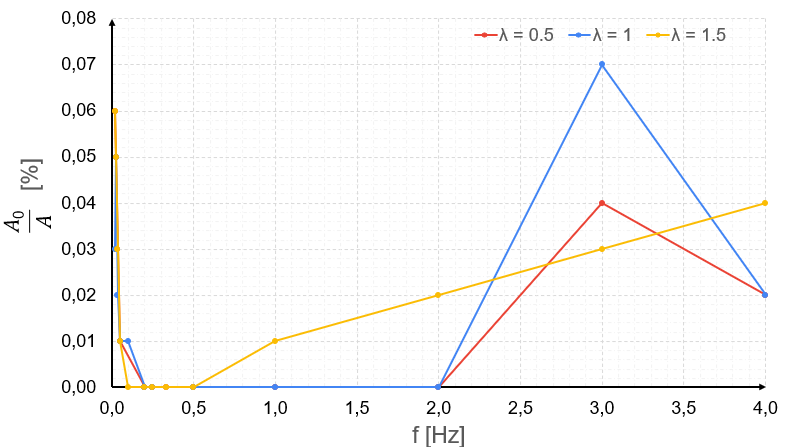
\includegraphics[width=1\linewidth]{../figs/1}
	\caption{Składowe zerowe dla różnych rzędów regulatorów członu $J_0$}
	\label{fig:1}
\end{figure}

\begin{figure}[ht]
	\centering
	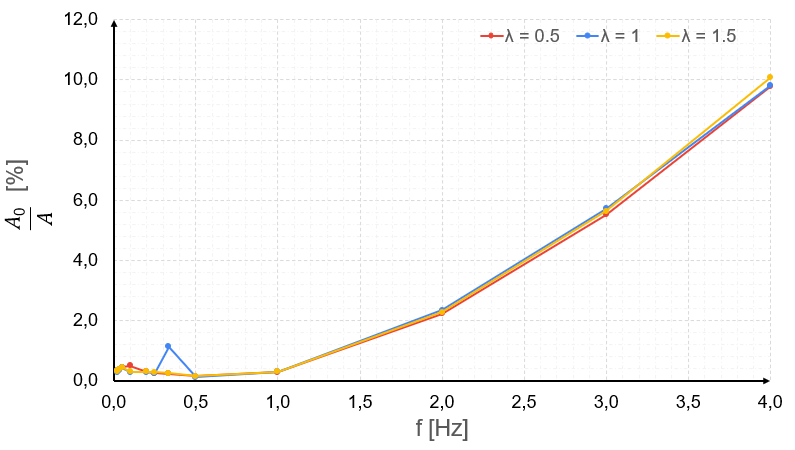
\includegraphics[width=1\linewidth]{../figs/2}
	\caption{Składowe zerowe dla różnych rzędów regulatorów członu $J_1$}
	\label{fig:2}
\end{figure}

\begin{figure}[ht]
	\centering
	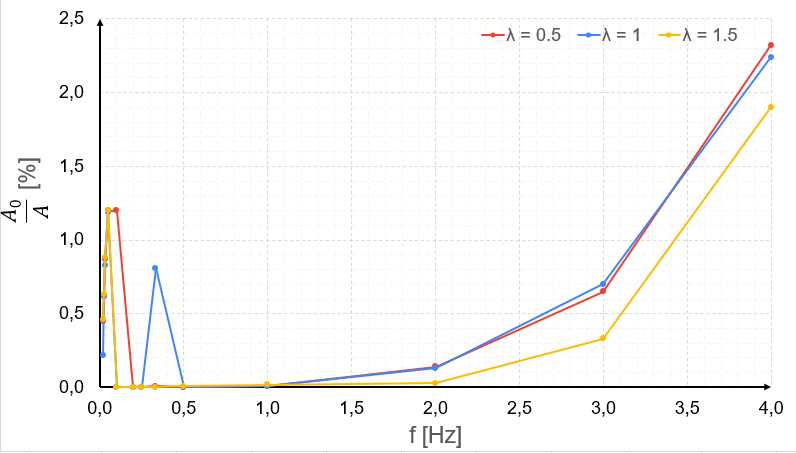
\includegraphics[width=1\linewidth]{../figs/3}
	\caption{Składowe zerowe dla różnych rzędów regulatorów członu $J_2$}
	\label{fig:3}
\end{figure}

\begin{figure}[ht]
	\centering
	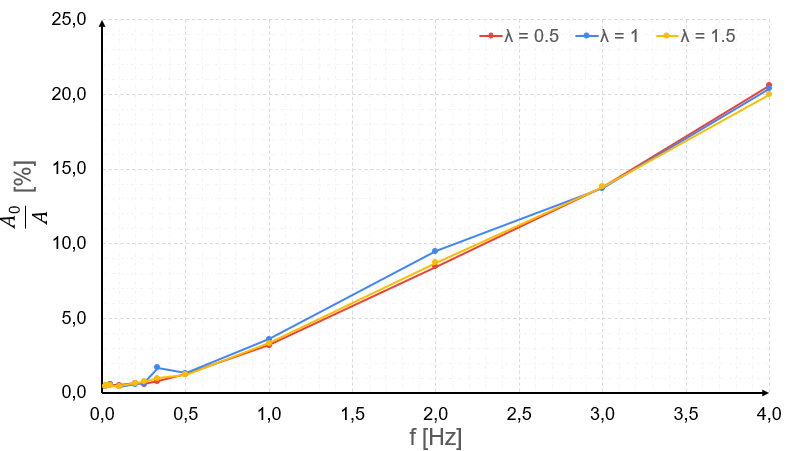
\includegraphics[width=1\linewidth]{../figs/4}
	\caption{Składowe zerowe dla różnych rzędów regulatorów członu $J_3$}
	\label{fig:4}
\end{figure}

\begin{figure}[ht]
	\centering
	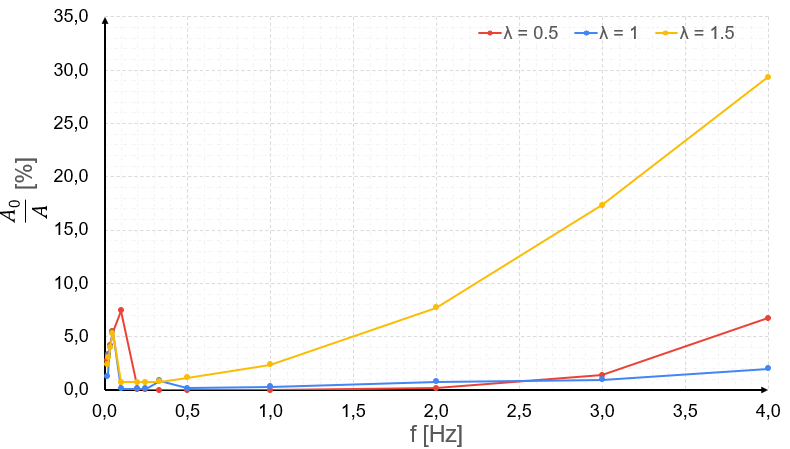
\includegraphics[width=1\linewidth]{../figs/5}
	\caption{Składowe zerowe dla różnych rzędów regulatorów członu $J_4$}
	\label{fig:5}
\end{figure}


\clearpage
\section{Bibliografia}
\begin{thebibliography}{00}
	\bibitem{matlab} Matlab - dokumentacja [Online]. Dostęp (22.11.2024 r.):
	\href{https://www.mathworks.com/help/matlab/}{https://www.mathworks.com/help/matlab/}
	
	\bibitem{simulink} Simulink - dokumentacja [Online]. Dostęp (22.11.2024 r.): \href{https://www.mathworks.com/help/simulink/}{https://www.mathworks.com/help/simulink/}
	
	\bibitem{Robotics Toolbox} Robotics Toolbox - dokumentacja [Online]. Dostęp (22.11.2024 r.):
	\href{https://www.mathworks.com/help/robotics/}{https://www.mathworks.com/help/robotics/}
	
	\bibitem{Simscape} Simscape - dokumentacja [Online]. Dostęp (22.11.2024 r.):
	\href{https://www.mathworks.com/help/robotics/}{https://www.mathworks.com/help/robotics/}
	
	\bibitem{FOMCON} A. Tepljakov, E. Petelnikov, and J. Belikov, "A flexible MATLAB tool for optimal fractional-order PID controller design subject to specifications," *Proc. 31st Chinese Control Conf.*, Hefei, China, Jul. 2012, pp. 4876–4881. [Online]. Dostęp (22.11.2024 r.): \href{https://www.researchgate.net/publication/259741861_A_Flexible_MATLAB_Tool_for_Optimal_Fractional-order_PID_Controller_Design_Subject_to_Specifications}{https://www.researchgate.net/publication/259741861}
	
	\bibitem{FOMCONdoc} FOMCON - dokumentacja [Online]. Dostęp (22.11.2024 r.):
	\href{https://fomcon.net/}{https://fomcon.net/}
	
	\bibitem{Hamachi} Hamachi - strona [Online]. Dostęp (22.11.2024 r.):
	\href{https://www.vpn.net/}{https://www.vpn.net/}
	
	\bibitem{Haguichi} Haguichi - instrukcja pobrania [Online]. Dostęp (22.11.2024 r.):
	\href{https://haguichi.net/download/}{https://haguichi.net/download/}
	
	\bibitem{ROS2} ROS2 foxy - dokumentacja [Online]. Dostęp (22.11.2024 r.):
	\href{https://docs.ros.org/en/foxy/index.html}{https://docs.ros.org/en/foxy/index.html}
	
	\bibitem{ROS Toolbox} ROS Toolbox - dokumentacja [Online]. Dostęp (22.11.2024 r.):
	\href{https://www.mathworks.com/help/ros/}{https://www.mathworks.com/help/ros/}
	
	\bibitem{Fractional}K. Rogowski, T. Kaczorek, "Fractional Linear Systems and Electrical Circuits",Studies in Systems, Decision and Control, Springer, NY, 2015
	
	\bibitem{Selected}T. Kaczorek, "Selected Problems of Fractional Systems Theory",Lecture Notes in Control and Information Sciences 411,  2011 Springer-Verlag Berlin Heidelberg
	
	\bibitem{Pawlusz}E. Pawłuszewicz, A. Koszewnik, P. Burzyński, "ON GRÜNWLAD-LETINKOV FRACTIONAL OPERATOR WITH MEASURABLE ORDER ON CONTINUOUS-DISCRETE TIME SCALE", acta mechanica et automatica, vol.14 no.3 (2020)
	
	\bibitem{Popolizio}M. Popolizio, "On the Matrix Mittag–Leffler Function: Theoretical Properties and Numerical Computation", Mathematics, 2019
	
	\bibitem{Kumar}Pushpendra Kumar, Dumitru Baleanu, Vedat Suat Erturk, Mustafa Inc and V. Govindaraj, "A delayed plant disease model with Caputo fractional derivatives", Advances in Continuous and Discrete Models, Springer, 2022
	
	\bibitem{falling}Mustafa Turkyilmazoglu, Mohamed Altanji, "Fractional models of falling object with linear and quadratic frictional forces considering Caputo derivative",Chaos, Solitons and Fractals, Elsevier, 2023
	
	\bibitem{plant}Muhammad Farman, Rabia Sarwar, Ali Akgul, "Modeling and analysis of sustainable approach for dynamics of infections in plant virus with fractal fractional operator", Chaos, Solitons and Fractals, Elsevier, 2023
	
	\bibitem{power}Georgios Tzounas, Ioannis Dassios,Mohammed Ahsan Adib Murad, and Federico Milano, "Theory and Implementation of Fractional Order Controllers for Power System Applications", IEEE TRANSACTIONS ON POWER SYSTEMS, VOL. 35, NO. 6, NOVEMBER 2020
\end{thebibliography}



\end{document}
